\documentclass[11pt, a4paper]{article}
\usepackage[utf8]{inputenc}
\usepackage[left=2cm, right=2cm, top=2.5cm, bottom=2.0cm]{geometry}
\usepackage{amsmath, amssymb, amsthm}
\usepackage[english]{babel}
\usepackage{graphicx}
\usepackage[font={small,it}]{caption}
\graphicspath{ {figures/} }
\usepackage{url}
\usepackage{appendix}
\usepackage{float}
\usepackage{multirow}
\usepackage[bottom]{footmisc}
\usepackage{wrapfig}
\usepackage{subcaption}
\usepackage{titling}
\setlength{\droptitle}{-10em}  

\title{ \huge Artificial neural networks \\ 
  { \large Assigment 4: PCA and SOM }}
\author{
        Lood, Cédric \\
        \small Master of Bioinformatics
}

\begin{document}
\maketitle
%\tableofcontents

\section{Context}

In this exercise session, I explored techniques of unsupervised
learning using neural networks.

\section{Principal component analysis}

\begin{figure}[H]
    \centering
    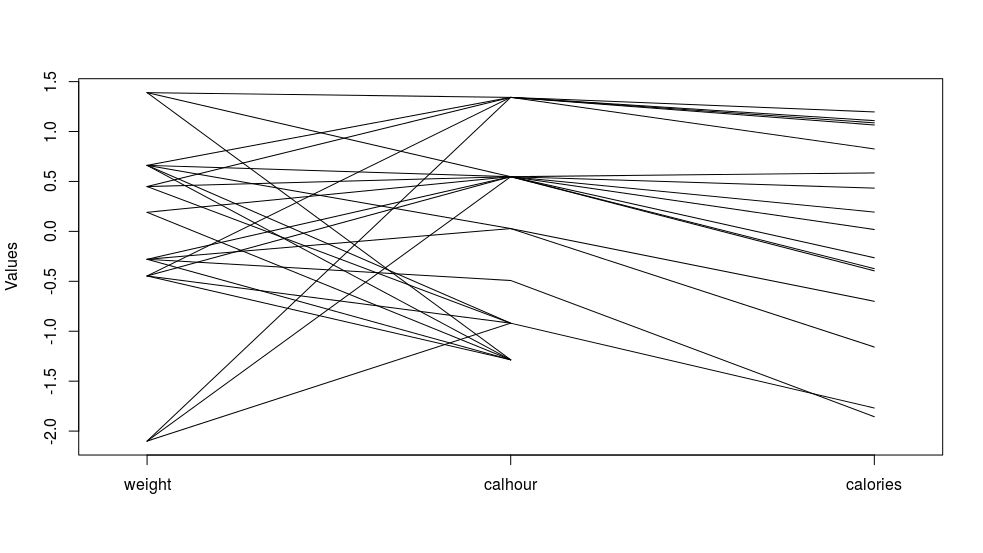
\includegraphics[scale=.55]{test.png}
    \caption{test}
    \label{fig:test}
\end{figure}


\bibliographystyle{ieeetr} 
\bibliography{bib-db}


\end{document}
